\chapter{System Implementation and Integration}
\label{System Implementation and Integration }

\section{Planning and constraint Module Implementation}
\label{Planning and constraint Module Implementation}

This chapter presents the technical realization of the constraints driven system architecture and algorithmic workflow introduced in chapter \ref{CH_3_System Concept and Methodology}. The previous chapter elaborated the methodological design of the system, the present chapter demonstrates how this methodology is implemented with an industrial robotic automation environment and convert the manual programming to automated programming robotic automation. The objective of this section is to define the development context, system boundaries, and integration structure within which the automatic robot program generation system operates.
\par The implementation is used inside an industrial robotic press brake cell. Such environment requires coordinated interaction between geometric reasoning, motion planning, robot control and peripheral device handling. Therefore, the system must not only execute validated motion sequence but must also ensure consistent synchronization between computational planning and physical robot execution.
\par From the system engineering perspective, the implementation is structured into three principal layers, a planning layer, an integration layer, and an execution layer. The planning layer contains rules based which are responsible for the orientation validation, grip determination, reachability assessment and strategy selection. The integration layer contains communication between the planning system and the robot control environment. The execution layer translates and validates the waypoint and functions to the physical robotic actions.
\par The separation between planning and execution is intentional and flows established modular automation principle, where decoupling decision – making from actuation improves system reliability and maintainability \cite{Thramboulidis2013MDE}. By maintaining this separation, the system ensures that constraints validation remain logically independent from motion execution. This ensures no motion is generated without geometric validation, grip stability and reachability conditions. The implementation environment provides motion primitives, coordinate management, and hardware abstraction through a controlled robotic framework. The planning system interfaces with this environment through a structured communication mechanism which enables the transfer of validated motion path. This structure allows automatic generation of robot programs with manual waypoint teaching, thereby replacing conventional teach pendant programming approaches discussed in Chapter\ref{CH_2_State of the Art}.
\par Simulation capability is incorporated with the implementation environment to enable pre-execution validation of all the decided trajectories. Simulation based validation and virtual commissioning are widely recognized as essential components of modern industrial robotic system deployment, as they allow execution logic to be verified prior to physical operation \cite{Bar2018VirtualCommissioning}. The integration of simulation into development workflow therefore supports robustness and reduces commissioning risk. The implemented process structured configuration inputs transformed them into validated geometric states and generated executable motion sequences through rule evaluation. Every execution is preceded by structural validation stages as defined in \ref{Algorithmic Implementation and Workflow}. This layered program ensures compliance with FR related to correct motion generation and NFR concerning predictable behavior.
The overall integration context of system is illustrated in Fig \ref{fig:integration_planning_anyrobot}, which shows the communication flow between the planning system and the robot control environment. The planning system generates validated motion paths based on the current state of the workpiece and the defined constraints. These paths are then transmitted to the robot control environment, which executes the corresponding robotic actions while ensuring synchronization with peripheral devices and safety monitoring systems.
\begin{figure}[htbp]
  \centering
  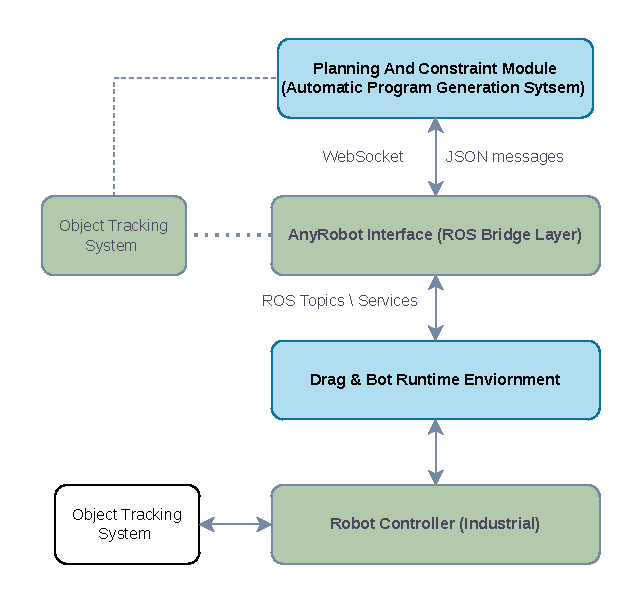
\includegraphics[
    width=\linewidth,
    height=0.45\textheight,
    keepaspectratio
  ]{figures/Integration_palnning_ch_4.pdf}
  \caption{Integration of planning system with AnyRobot Interface}
  \label{fig:integration_planning_anyrobot}
\end{figure}

From a development standpoint, the system is implemented with emphasis on execution and explicit state control. No learning-based mechanisms are used, while all the decisions are governed under constraint conditions. This design simplifies validation in an industrial automation context where predictable behavior is mandatory.
In summary, this section established the technical integration framework within which the automatic robot program robotic system operates. The following section details the realization of individual functional components, beginning with the robot control environment and communication interface.


\subsection{Layered Software Architecture Realization}
\subsection{Layered Software Architecture Realization}
As introduced, in chapter 3, the system architecture is structured into three principal layers, a planning and constraint layer, an integration layer and a execution layer. In this section, the focus is not on conceptual justification of this structure, but on its realization within the implemented system. The layered structure was implemented to ensure separations between the validation logic, communication handling and physical robot execution. This separation guarantees that the motion generation remains independent from control specific execution states.(may be remove this section) %%%%%%%%%%%%%%%%% May be removing this section 
